Solar energy has the momentum to replace fossil fuels in the green transition and to keep it going the discovery of more efficient photovoltaic materials is necessary. Core spectroscopy has long been used to elucidate the electronic structure of materials. It is not new, but the ability to do this on an attosecond time scale is, as evidenced by the Nobel Prize in 2023. Such a short time scale lends high resolution to molecular processes, which allows for the design of improved solar materials. 
\begin{wrapfigure}{r}{0.5\textwidth}
   \centering
   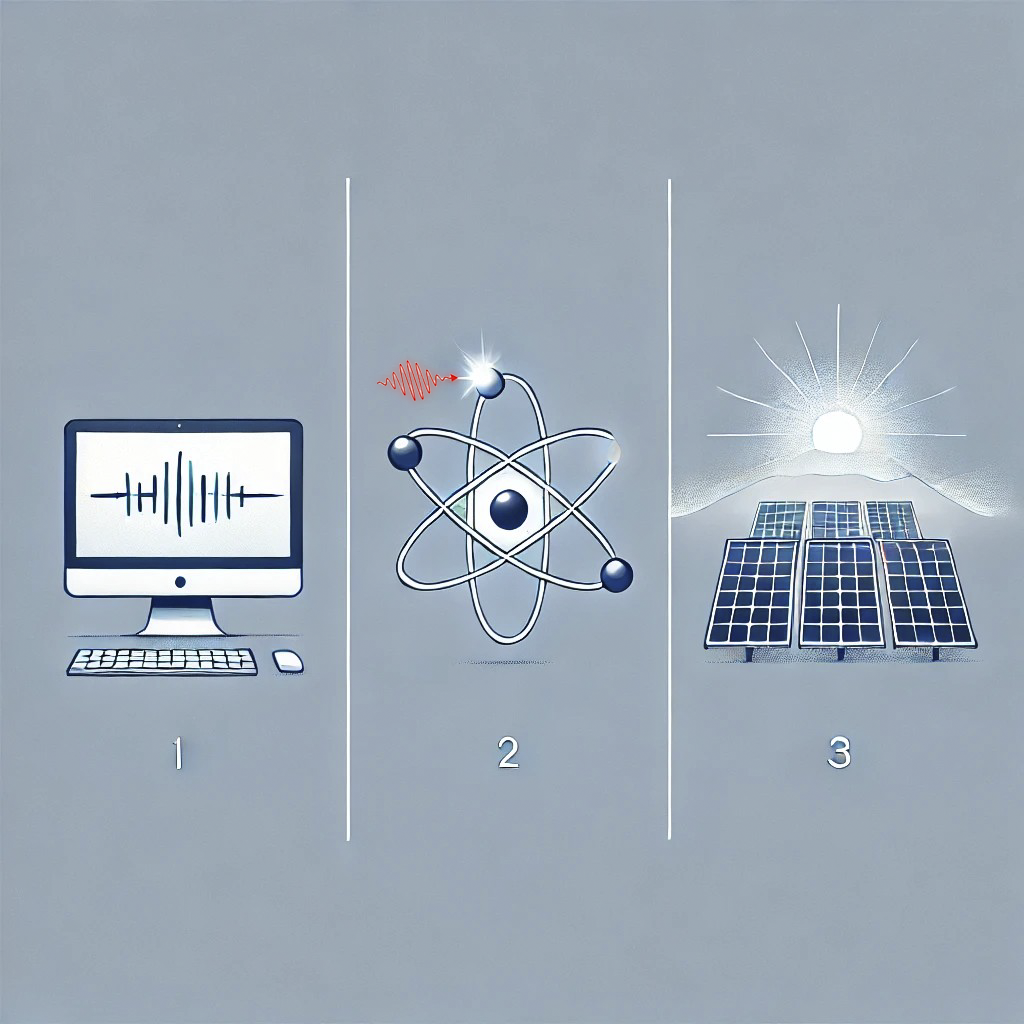
\includegraphics[width=0.4\textwidth]{picture.png}
   \caption{(1) The development of computational methodologies (2) elucidates the core spectroscopy of materials to (3) produce more efficient solar cells.}
   \label{fig:fig1}
\end{wrapfigure}
Computation guides these experiments, as exemplified by the workflow of Figure \ref{fig:fig1}. Density Functional Theory (DFT) has long served as the computational workhorse of materials science, due to its reasonable accuracy at low expense. However, it treats the repulsive interactions between electrons using an approximate exchange-correlation functional, leading to variable results with a lack of systematic improvability \cite{kozlowski_elucidating_2021}. A potential solution is the application of Green's functions in many-body perturbation theory (MBPT). Central is the Dyson equation,
\begin{equation}
G = G_0 + G_0 \Sigma G,
\label{eqn:dyson}
\end{equation}
which relates the Green's function of the fully interacting system \( G \) to that of the non-interacting system \( G_0 \) through the self-energy \( \Sigma \). The self-energy \( \Sigma \) is designed to capture the many-body interactions neglected by \( G_0 \). Hedin provided a closed set of 5 equations that can be used to obtain \( G \) and \( \Sigma \). In the common \( GW \) approximation, the self-energy \( \Sigma \) takes the form \( iGW \), where \( W \) is the screened Coulomb interaction. Various levels of self-consistency can be done within \( GW \); the highest level is fully self-consistent \( GW \) (sc\( GW \)). Even at the high computational expense of scGW, the scheme often does not deliver improved results over the lower levels of self-consistency. To remedy this, one has to include vertex corrections beyond the \( GW \) approximation \cite{kutepov_one-electron_2017}, which is computationally intensive. The root of these issues is that Hedin's equations solve for the self-energy \( \Sigma \) through a perturbative expansion in the interaction strength \( W \). The \( GW \) approximation is accurate for weakly correlated systems where this expansion is reasonable, but it is not for the strongly correlated, where the interaction is large.

The Mori-Zwanzig (MZ) theory offers an alternative. Originating from statistical physics, one starts from a similar Dyson equation \ref{eqn:dyson}, but the self-energy \( \Sigma \) is replaced by a memory kernel. This memory kernel is now expanded in powers of the evolution time \( t \), making the Dyson series expansion with MZ converge faster for strongly correlated systems. Recently, a diagrammatic theory for MZ with Green's functions has been introduced in the form of tree diagrams \cite{zhu_combinatorial_2022}, as opposed to the Feynman diagrams of \( GW \). To date, however, no computational implementation has been done and the proposed work will address this gap.